\vspace{-0.1in}
\section{Future Directions}
\label{sec:future}
\vspace{-0.05in}

So far, we used emulation and simulation to evaluate the minimum network requirements for  disaggregation.%, with a focus on minimizing degradation in application performance. 
This opens two directions for future work: (1) demonstrating an end-to-end system implementation of remote memory access that meets our latency targets, and (2) investigating programming models that actively exploit disaggregation to \emph{improve} performance.
We present early results investigating the above with the intent of demonstrating the potential for realizing positive results to the above questions: each topic merits an in-depth exploration that is out of scope for this paper.


\vspace{-0.1in}
\subsection{Implementing remote memory access}
\vspace{-0.05in}
We previous identified an end-to-end latency target of 3-5us for \dis that we argued could be met with RDMA. The (promising) RDMA latencies in \S\ref{sec:existing} are as reported by native RDMA-based applications. 
We were curious about the feasibility of realizing these latencies if we were to retain our 
architecture from the previous section in which remote memory is accessed as a special swap device as this would provide a simple and transparent approach to utilizing remote memory. 

We thus built a kernel space RDMA block device driver which serves as a swap device; i.e., the local CPU can now swap to remote memory instead of disk.
We implemented the block device driver on a machine with Mellanox  4xFDR Infiniband card.
We test the block device throughput using \textit{dd} with direct IO, and measure the request latency by instrumenting the driver code. 
The end-to-end latency of our approach includes the RDMA request latency and the latency introduced by the kernel swap itself. We focus on each in turn. 

\paragraph{RDMA request latency.} A few optimizations were necessary to improve RDMA performance in our context. First, we \emph{batch} block requests sent to the RDMA NIC and the driver waits for all the requests to return before notifying the upper layer: this gave a block device throughput of only 0.8GB/s and latency around 4-16us.
Next, we \emph{merge} requests with contiguous addresses into a single large request: this improved throughput to 2.6GB/s (a ~3x improvement).
Finally, we allow \emph{asynchronous} RDMA requests: we created a data structure to keep track of outgoing requests and notify the upper layer immediately for each completed request; this improves throughput to 3.3GB/s which is as high as a local RamFS, and reduces the request latency to 3-4us (Table \ref{tab:rdma_latency}). 
This latency is within 2x of latencies reported by native RDMA applications which we view as encouraging given the simplicity of the design and that additional optimizations are likely possible.

\begin{table}[t]
    \centering
    \small
    \begin{tabular}{ccccc}
    \textbf{Min}	& \textbf{Avg}	& \textbf{Median} & \textbf{99.5 Pcntl}	& \textbf{Max}\\
    \hline
    3394 &	3492&	3438&	4549&	12254\\\hline
    \end{tabular}
    \caption{RDMA block device request latency(ns)}
    \label{tab:rdma_latency}
\end{table}



\eat{
The RDMA block device driver provides us a simple and efficient way utilize remote memory. 
We setup the block device as swap space and run the \rc{5} applications evaluated in \S \ref{sec:requirements} with lower latency requirements.
\rc{waiting for joao's results}

}

%We also could not arbitrarily introduce
%\texttt{printk} calls within the areas we were measuring, since \texttt{printk}
%introduces a noticable overhead when measuring on the order of microseconds.
% (as evidenced by the \texttt{VM\_FAULT\_*} macros in the \texttt{mm.h} header). 
\paragraphb{Swap latency}
We calculated the software overhead of swapping on a commodity desktop running Linux 3.13 by simultaneously measuring the times spent in the page fault handler and accessing disk. 
We found that convenient measurement tools such as \texttt{ftrace} and \texttt{printk} introduce unacceptable overhead for our purposes. 
%Instead, we took advantage of the fact that the
%\texttt{handle\_mm\_fault} function called by the page fault handler (and which eventually handles swaps) never utilizes the upper 16 bits of its 32 bit return value.
Thus, we wrap both the body of the \texttt{\_\_do\_page\_fault} function and the call to the \texttt{swapin\_readahead} function (which performs a swap from disk) in \texttt{ktime\_get} calls.  
We then pack the result of the measurement for the \texttt{swapin\_readahead} function into the unused upper 16-bits of the return value of its caller, \texttt{do\_swap\_page}, which propagates the value up to \texttt{\_\_do\_page\_fault}. 

Once we have measured the body of \texttt{\_\_do\_page\_fault}, we record both the latency of the whole \texttt{\_\_do\_page\_fault} routine, as well as the time spent in
\texttt{swapin\_readahead}. 
We subtract these and average to find that the
software overhead of swapping is 2.47 $\mu$s. 
This number is a lower-bound on the software overhead of the handler, because we assume that all of \texttt{swapin\_readahead} is a ``disk access''.% (we cannot neatly instrument inside \texttt{swapin\_readahead} in the same manner since it returns a pointer).

In combination with the above RDMA latencies, these early numbers suggest that a simple system design for low-latency access to remote memory could be realized. 

\eat{ 

, there is likely room for optimization: in current non-NUMA architectures, the Linux Kernel only launches one \textit{kswapd} to swap out least recently used pages which could be a bottleneck for 
This could be a bottleneck for apps that heavily use remote memory.
We enable the NUMA\_EMU feature in Linux kernel, which partitions the memory into several regions, and each memory region gets its own \textit{kswapd}. 
This improves the throughput of swapping out memory pages.
}

%Overall, our measurement code introduces a very small number of bitwise
%operations (ANDs, ORs, shifts), one integer subtraction, and four calls to
%\texttt{ktime\_get} into the handler, which together have a negligible impact on
%measurements.
\subsection{Improved performance via disaggregation}
%Our study so far has focused on characterizing the network requirements for \dis that would lead to little or no performance degradation in existing applications. However,
In the longer term, one might expect to re-architect applications to actively exploit disaggregation for improved performance.
One promising direction is for applications to exploit the availability of low-latency access to large pools of remote memory~\cite{ddcHwDesign1}. 
One approach to doing so is based on extending the line of argument in the COST work~\cite{cost} by using remote memory to avoid parallelization overheads.
% cite hotnets, reiss??
We estimate the potential benefits of this approach, with the following experiment .
%to show that applications adapted to disaggregated environment can outperform traditional server centric ones.
First, to model an application running in a \dis, we set up a virtual machine with 4 cores,  2GB of local memory, and access to an ``infinitely'' large remote memory pool by swapping to an RDMA-backed block device. 
%This is considered as a simulation to running apps in \dis.
Next, we consider two scenarios that represent server-centric architecture.
One is a server with 4 cores and 8GB of local memory (25\% larger than the \dis case as in previous sections) and an ``infinitely'' large local SSD swap -- this represents the COST baseline in a server-centric context. 
Second, we evaluate GraphX using a 16-node m2.4x large cluster on EC2 -- this represents the scale-out approach in current server-centric architecture.
We run Pagerank and Connected Components using COST, a single-thread graph compute engine over three large graph datasets. COST mmaps the input file, so we store the input files on another RDMA-backed block device.
Figure \ref{fig:benefit} shows the application runtime of COST-DDC, COST-SSD and GraphX-Server Centric.
In all but one case, COST-DDC is 1.48 to 2.05 times faster than the GraphX (server-centric) scenario and slightly better than the server-centric COST scenario (the improvement over the latter grows with increasing data set size). Performance is worse for Pagerank on the UK-2007-5 dataset, consistent with the results in ~\cite{cost} because the graph in this case is more easily partitioned. 



Finally, another promising direction for improving performance is through better resource utilization. As argued in~\cite{hotnets, ddcHwDesign1}, CPU-to-memory utilization for tasks in today’s datacenters varies by three orders of magnitude across tasks; by `bin packing' on a much larger scale, \dis should achieve more efficient statistical multiplexing, and hence higher resource utilization and improved job completion times. We leave an exploration of this direction to future work. 


\begin{figure}
  \centering
    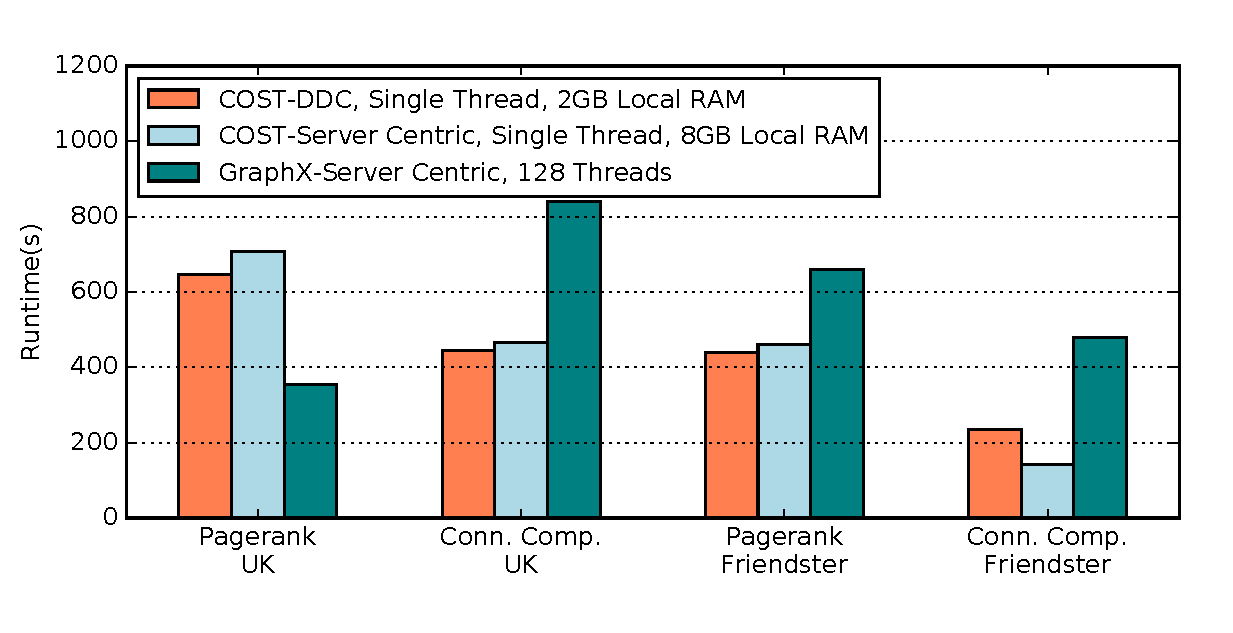
\includegraphics[width = \columnwidth]{img/benefit_uk.eps} 
  \caption{\small{Running COST in a simulated DDC. COST-DDC is 1.48 to 2.05 faster than GraphX-Server Centric except for one case. We use two datasets in our evaluation, UK-2007-05 (105m nodes, 3.7b edges), and Friendster (65m nodes, 1.8b edges)}}
  \label{fig:benefit}
\end{figure}
